\section{Electron and Photons}
\label{sec:reco:EM}

\subsection{Electron and Photon Reconstruction}
\label{sec:EM:reco}

\indent Both electron and photon reconstruct starts from clusters of energy deposits in the electromagnetic calorimeter.  The EM calorimeter is first divided into a grid of towers each with the size of $\Delta \eta \times \Delta \phi = 0.025 \times 0.025$.  The energy of all cells in the longitudinal layers inside each tower is summed into the total tower energy.  \\

\indent The EM clusters are seeded by towers with energy above a certain threshold.  A sliding-window algorithm then groups the energy towers near the seed into EM clusters.\cite{EMReco13TeV,EMReco8TeV}  The window width is $3 \times 7$ towers in the barrel and $5 \times 5$ towers in the endcap.  The reconstructed cluster therefore has a size of $\Delta \eta \times \Delta \phi = 0.075 \times 0.175$ in the barrel and $ 0.125 \times 0.125$ in the endcap.  The same window size is used for electrons and photons to ensure better cancelation of systematics when using electrons to measure photon response.\cite{EMReco13TeV}  The window position is adjusted so that the reconstructed cluster energy is the local maximum.  The different cluster sizes were optimized for the different energy distribution in the barrel and endcap calorimeters while minimizing pileup and noise contributions.\cite{EMReco13TeV}  \\

\indent Identified clusters are then matched to reconstructed ID track using track and cluster position.  ID tracks are required to have a minimum number of pixel and total silicon hits.  Clusters are considered an electron candidate if a single well-reconstructed ID track that originates from a vertex is found.  The cluster is considered an unconverted photon candidate if no tracks are found.  The cluster is considered a converted photon candidates if two opposite signed tracks that are collinear, originate from the interaction point, and are consistent with electrons are present.  The cluster if also considered a converted photon if a single track is present but the track lacks hits in the IBL of the pixel detector.  \\

\indent Furthermore, electron and photon candidates must satisfy a set of criteria.  These variables include descriptions of the EM shower shapes, amount of hadronic activity behind the EM calorimeter and properties of associated tracks.  More details on electron and photon identification are given in section \ref{sec:reco:eleQuality} and \ref{sec:reco:phoQuality}. \\

\subsection{Electron Identification and Quality}
\label{sec:reco:eleQuality}

\indent Electron identification in Run 2 is based on a likelihood algorithm that depends on a list of kinematics variables including EM shower shape, EM vs hadronic activity ratio, activity in the TRT and properties of the associated track.  The list of variables included in the likelihood can be found in \cite{EleID}.  A multivariate technique is used to ensure the PDF estimation is robust in low statistics regions in the high dimensional space.  Probability density functions (PDF) are formed for electrons and non-electron backgrounds for a set of discriminating variables used on MC.  The probability of the candidate being an electron is calculated using the two PDFs.  \\

%TypeDescriptionNameHadronic leakageRatio ofETin the first layer of the hadronic calorimeter toETof the EM clusterRhad1(used over the range|?|<0.8 or|?|>1.37)Ratio ofETin the hadronic calorimeter toETof the EM clusterRhad(used over the range 0.8<|?|<1.37)Back layer ofRatio of the energy in the back layer to the total energy in the EM accordionf3EM calorimetercalorimeter. This variable is only used below 100 GeV because it is known tobe inefficient at high energies.Middle layer ofLateral shower width,q(?Ei?2i)/(?Ei)?((?Ei?i)/(?Ei))2, whereEiis thew?2EM calorimeterenergy and?iis the pseudorapidity of celliand the sum is calculated withina window of 3�5 cellsRatio of the energy in 3�3 cells over the energy in 3�7 cells centered at theR?electron cluster positionRatio of the energy in 3�7 cells over the energy in 7�7 cells centered at theR?electron cluster positionStrip layer ofShower width,p(?Ei(i?imax)2)/(?Ei), whereiruns over all strips in a windowwstotEM calorimeterof??�???0.0625�0.2, corresponding typically to 20 strips in?, andimaxis the index of the highest-energy stripRatio of the energy difference between the largest and second largest energyEratiodeposits in the cluster over the sum of these energiesRatio of the energy in the strip layer to the total energy in the EM accordionf1calorimeterTrack conditionsNumber of hits in the innermost pixel layer; discriminates againstnBlayerphoton conversionsNumber of hits in the pixel detectornPixelNumber of total hits in the pixel and SCT detectorsnSiTransverse impact parameter with respect to the beam-lined0Significance of transverse impact parameter defined as the ratio ofd0d0/?d0and its uncertaintyMomentum lost by the track between the perigee and the last?p/pmeasurement point divided by the original momentumTRTLikelihood probability based on transition radiation in the TRTeProbabilityHTTrack-cluster??between the cluster position in the strip layer and the extrapolated track??1matching??between the cluster position in the middle layer and the track extrapolated??2from the perigeeDefined as??2, but the track momentum is rescaled to the cluster energy??resbefore extrapolating the track from the perigee to the middle layer of the calorimeterRatio of the cluster energy to the track momentumE/p6

\indent Electron identification is split into categories {\it very loose, loose, medium, } and {\it tight}.  Each operating point is a sub-set of another.  For example, all tight electrons are also medium electrons and so on.  25 GeV tight electrons have an efficiency of 78 percent and fake rate of 0.3 percent.  25 GeV loose electrons have an efficiency of 90 percent and fake rate of 0.8.  The efficiency increases with $E_T$ while the fake rate decreases.\cite{EleID} \\

\indent Because some shower shape distributions tend to broaden with the number of pileup collisions, the cut on the likelihood discriminant is loosened as a function of the number of vertices. This is done to preserve the identification efficient at high pileup and does not drastically increase the amount of background.\cite{EleID} 

\subsection{Photon Identification and Quality}
\label{sec:reco:photoID}

\indent Photon identification is based on the shower shape and the amount of hadronic activity behind the EM cluster.  The energy deposited in the cells in the first and second layer of the EM calorimeter are important for distinguishing the EM shower originating from photons and those originating the neutral mesons such as $\pi_0$. A detailed list of the discriminating variables used can be found in \cite{photonID}. \\

\indent The requirements are different for converted and unconverted photon candidates to account for the different expected shower shapes.  The requirements are differ in pseudorapidity intervals to account for the varying amount of material upstream of the calorimeter. The requirements were optimized using a multivariate technique.\cite{TMVA}\\

\indent Two working points are included a loose and a tight selection.  The loose ID exploits the variables only in the EM calorimeter and in the hadronic calorimeter layer and is typically used for the trigger and for background studies.  The tight ID uses the full granularity of the EM calorimeter, including the fine segmentation of the first sampling layer, and tightens requirements on the variables used in the loose selection.  The tight working point is the one generally recommended for physics analysis and photons used in this analysis are tight photons.  \\

%CategoryDescriptionNameloosetightAcceptance|?|<2.37, with 1.37<|?|<1.52 excluded??   ?Hadronic leakageRatio ofETin the first sampling layer of the hadroniccalorimeter  toETof  the  EM  cluster  (used  over  therange|?|<0.8 or|?|>1.37)Rhad1?   ?Ratio ofETin the hadronic calorimeter toETof theEM cluster (used over the range 0.8<|?|<1.37)Rhad?   ?EM Middle layerRatio of 3�7?�?to 7�7 cell energiesR??   ?Lateral width of the showerw?2?   ?Ratio of 3�3?�?to 3�7 cell energiesR??EM Strip layerShower width calculated from three strips around thestrip with maximum energy depositws3?Total lateral shower widthwstot?Energy outside the core of the three central strips butwithin seven strips divided by energy within the threecentral stripsFside?Difference  between  the  energy  associated  with  thesecond maximum in the strip layer and the energy re-constructed in the strip with the minimum value foundbetween the first and second maxima?E?Ratio  of  the  energy  difference  associated  with  thelargest and second largest energy deposits to the sumof these energiesEratio?Table 2: Discriminating variables used forlooseandtightphoton identification.20


\subsection{Electron and Photon Energy Calibration}
\label{sec:reco:EMCalibration}

\indent Electron and photon energy must also be calibrated because of the non-compensating nature of the EM calorimeter.  At the same time, the correctly estimating the amount of material upstream of the calorimeter is also important.  Typically a $100 \gev$ electron will deposit between a few percent to 20 percent of its energy before it reaches the calorimeter.\cite{EMReco13TeV} Also about 5 percent of the electron energy may be deposited outside of the cluster.  Electron and photon calibration accounts for all these affects to get an estimate of the true electron and photon energy.  The calibration procedure follow the steps indicated in figure \ref{fig:EMCalibFlow}.

\begin{figure}[htb]
  \begin{center}
    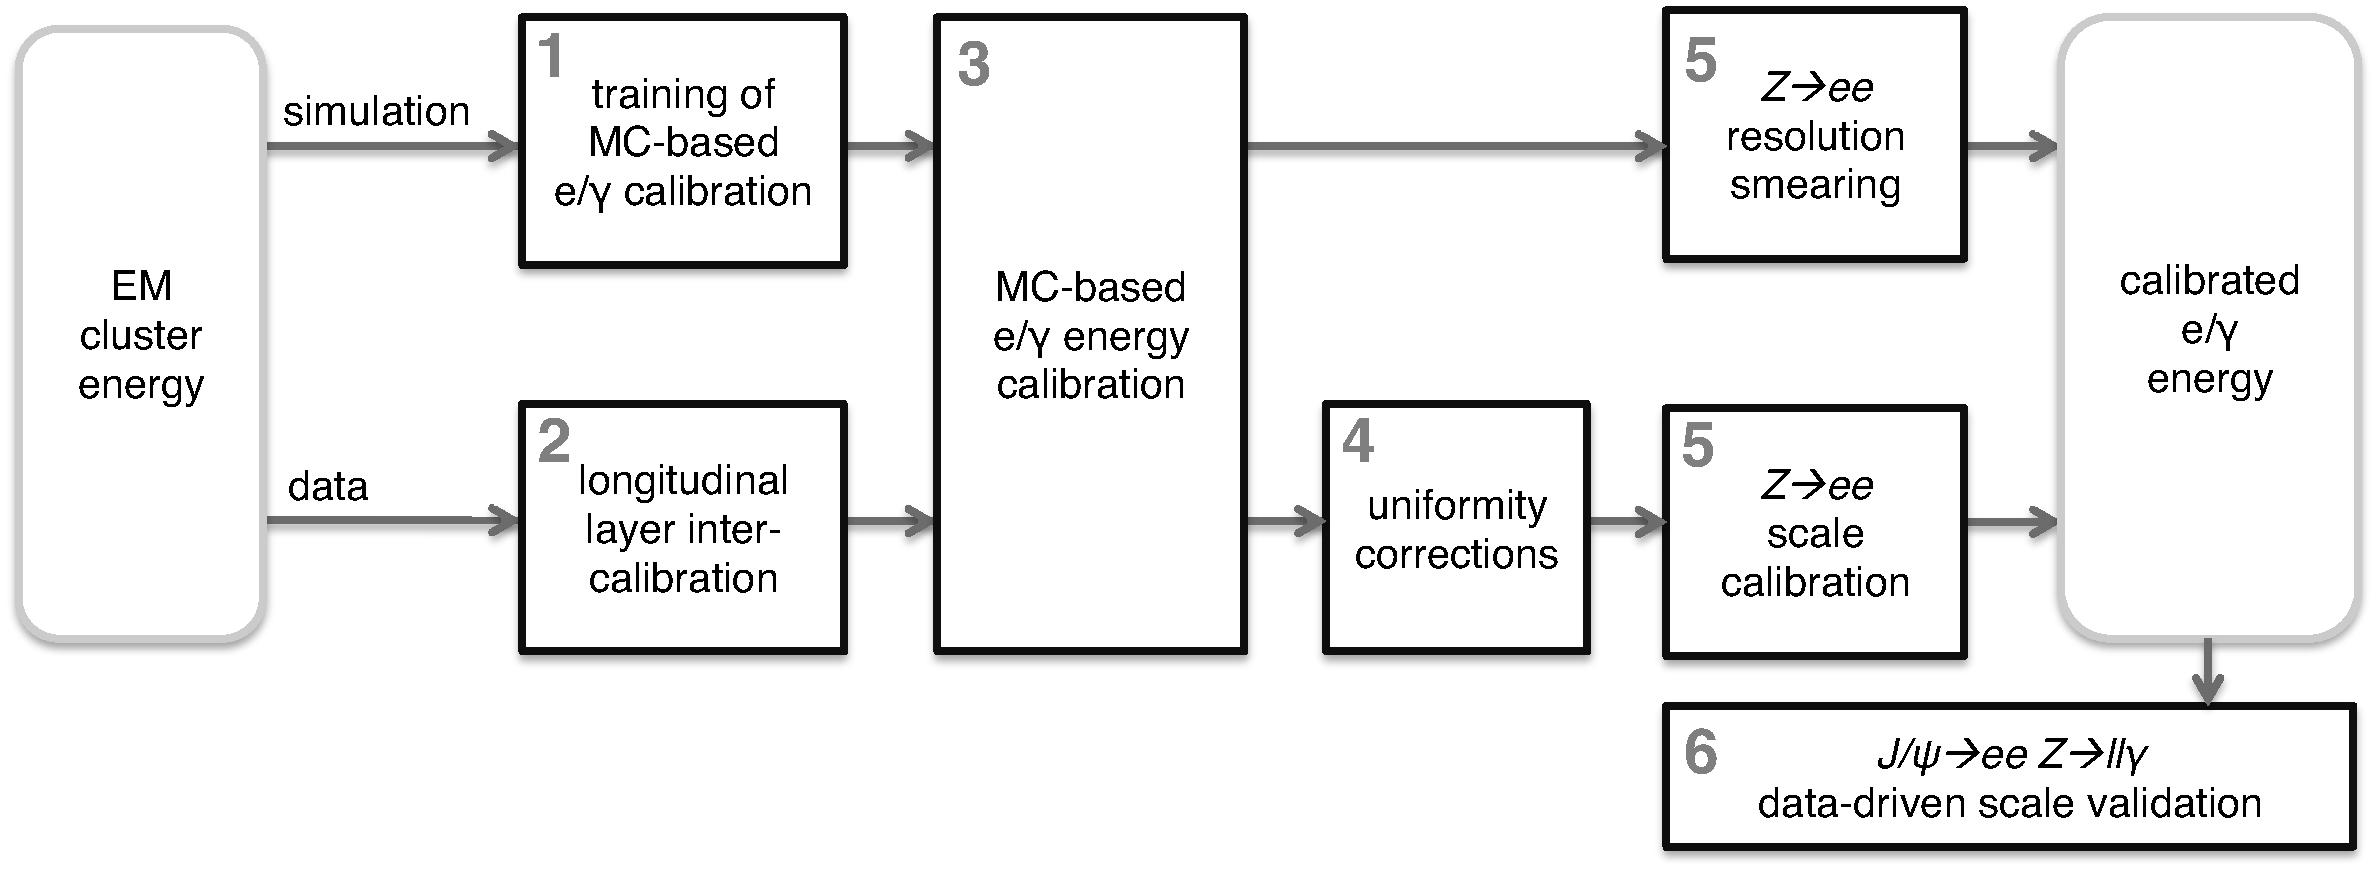
\includegraphics[width=0.85\textwidth]{figures/EMCalib/ElecCalib.png}\hspace{0.05\textwidth}
\end{center}
\caption{Flow chart of the steps involved in the calibration of the energy response of electrons and photons \cite{EMReco8TeV}}
\label{fig:EMCalibFlow} 
\end{figure}

\indent The EM clusters are first calibrated to the original electron or photon energy using a multivariate technique \cite{TMVA} based on MC simulations.\cite{EMReco13TeV,EMReco8TeV}   The MC based calibration uses information on the EM cluster properties such as the longitudinal shower shape and information from any associated ID track.  The response is different for electrons, converted photons and unconverted photons.  \\

\indent The longitudinal layers of the EM calorimeter must be calibrated relative to one another.  Specifically, the relative energy response of the presampler and the first and second layer must be validated by using data.  These cannot be done at the cluster level as clusters sum over all longitudinal layers.  The intercalibration of the first and second layers of the EM calorimeter is performed with $Z\rightarrow\mu\mu$ decays.   This is because the muon energy deposit in the calorimeter are relatively insensitive to the amount of material upstream of the EM calorimeter  The presampler energy scale is calibrated using W and Z decays.  The ratio of data to MC in the presampler energy detected in electrons from W and Z to electron decays is used as a scale factor.  This accounts for mismodeling of the amount of material in front of the presampler. \\

\indent A number of corrections are then applied to account for differences between simulation and data such as regions with non-optimal HV and geometrical affects.  Finally a correction is applied to ensure that the $Z\rightarrow ee$ modeling in simulation agrees with data.  The same scale factors derived for electrons from $Z\rightarrow ee$ is applied to photons but additional photon-specific systematic uncertainties are also applied.  \\

\indent Cross-checks of the electron and photon calibration is performed with $J/\psi \rightarrow ee$ and $Z \rightarrow ll\gamma$ events in data after all energy corrections are applied.  